%% LyX 2.0.3 created this file.  For more info, see http://www.lyx.org/.
%% Do not edit unless you really know what you are doing.
\documentclass[english]{beamer}
\usepackage[T1]{fontenc}
\usepackage[latin9]{inputenc}
\setcounter{secnumdepth}{3}
\setcounter{tocdepth}{3}
\usepackage{color}
\usepackage{bm}
\usepackage{amsmath,amsfonts,amssymb,mathrsfs}
\usepackage{graphicx}
\usepackage{esint}
\usepackage{subfigure} 
\usepackage{algorithm}
\usepackage{algorithmic}

\makeatletter

%%%%%%%%%%%%%%%%%%%%%%%%%%%%%% LyX specific LaTeX commands.
%% A simple dot to overcome graphicx limitations
\newcommand{\lyxdot}{.}
\newcommand{\bfu}[1]{\underline{\bf {#1}}}

%%%%%%%%%%%%%%%%%%%%%%%%%%%%%% Textclass specific LaTeX commands.
 % this default might be overridden by plain title style
 \newcommand\makebeamertitle{\frame{\maketitle}}%
 \AtBeginDocument{
   \let\origtableofcontents=\tableofcontents
   \def\tableofcontents{\@ifnextchar[{\origtableofcontents}{\gobbletableofcontents}}
   \def\gobbletableofcontents#1{\origtableofcontents}
 }
 \long\def\lyxframe#1{\@lyxframe#1\@lyxframestop}%
 \def\@lyxframe{\@ifnextchar<{\@@lyxframe}{\@@lyxframe<*>}}%
 \def\@@lyxframe<#1>{\@ifnextchar[{\@@@lyxframe<#1>}{\@@@lyxframe<#1>[]}}
 \def\@@@lyxframe<#1>[{\@ifnextchar<{\@@@@@lyxframe<#1>[}{\@@@@lyxframe<#1>[<*>][}}
 \def\@@@@@lyxframe<#1>[#2]{\@ifnextchar[{\@@@@lyxframe<#1>[#2]}{\@@@@lyxframe<#1>[#2][]}}
 \long\def\@@@@lyxframe<#1>[#2][#3]#4\@lyxframestop#5\lyxframeend{%
   \frame<#1>[#2][#3]{\frametitle{#4}#5}}
 \def\lyxframeend{} % In case there is a superfluous frame end
 \long\def\lyxplainframe#1{\@lyxplainframe#1\@lyxframestop}%
 \def\@lyxplainframe{\@ifnextchar<{\@@lyxplainframe}{\@@lyxplainframe<*>}}%
 \long\def\@@lyxplainframe<#1>#2\@lyxframestop#3\lyxframeend{%
   \frame<#1>[plain]{\frametitle{#2}#3}}

%%%%%%%%%%%%%%%%%%%%%%%%%%%%%% User specified LaTeX commands.
\usepackage{listings}
\usepackage{graphicx}
\usepackage{psfrag}
\usetheme{Warsaw}
\setbeamercovered{transparent}
\newcommand\ci{\protect\mathpalette{\protect\cI}{\perp}}
\def\cI#1#2{\mathrel{\rlap{$#1\;#2$}\mkern2mu{#1#2\;}}}

\usepackage{pgf}\usepackage{pgfarrows}\usepackage{pgfnodes}\usepackage{pgfautomata}\usepackage{pgfheaps}\usepackage{pgfshade}%\usepackage{beamerthemeshadow}
\usepackage{colortbl}%\usepackage{natbib}

\renewcommand{\Re}{\mathbb{R}}

\definecolor{dred}{rgb}{0.9,0.3,0.1}
\definecolor{blue}{rgb}{0.1,0.1,0.9}


\makeatletter

%colours
\definecolor{red}{rgb}{0.8,0.2,0.2}
\newcommand{\todo}[1]{{\color{red} {#1}}}

%environment
%\newcommand{\remark}{{\bm Remark.}}
\newcommand{\defn}{{\bf defn.\ }}

\newcommand{\I}{\mathbb{I}}
\newcommand{\R}{\mathbb{R}}
\newcommand{\Z}{\mathbb{Z}}
\renewcommand{\P}{\mathbb{P}}
\newcommand{\Q}{\mathbb{Q}}
\newcommand{\E}{\mathbb{E}}
\newcommand{\C}{\mathbb{C}}
\newcommand{\N}{\mathbb{N}}

\newcommand{\dataA}{\cD_A}
\newcommand{\dataB}{\cD_B}
\newcommand{\dataC}{\cD_C}
\newcommand{\voted}{\text{\sc voted}}
\newcommand{\spine}{{\cP_{\rm spine}}}
\newcommand{\data}{{\rm data\ }}
\newcommand{\MAP}{{\rm MAP}}
\newcommand{\interpolant}{\text{\sc interpolant}}
\newcommand{\samp}{\mathcal{S}}
\newcommand{\init}{{\rm init}}
\newcommand{\fin}{{\rm fin}}

%roman text
\newcommand{\labelled}{{\rm labelled}}
\newcommand{\unlabelled}{\rm unlabelled}
\newcommand{\normal}{\rm norm}

%metric spaces
\newcommand{\comp}{\overline}


%punctuation
\newcommand{\EQindent}{\ \ \ \ \ \ \ }
\newcommand{\ls}{``}
\newcommand{\wh}{\widehat}
\newcommand{\what}{\wh}
\newcommand{\wtilde}{\widetilde}
\newcommand{\bslash}{\backslash}

%equations
\newcommand{\bqan}{\begin{eqnarray*}}
\newcommand{\eqan}{\end{eqnarray*}}
\newcommand{\bqa}{\begin{eqnarray}}
\newcommand{\eqa}{\end{eqnarray}}
\newcommand{\bga}{\begin{align}}
\newcommand{\ena}{\end{align}}
\newcommand{\nn}{\nonumber}

%Linear Algebra and Operations
\newcommand{\diag}{{\rm diag}}
\newcommand{\row}{{\rm row}}
\newcommand{\col}{{\rm col}}
\newcommand{\lnull}{{\rm leftnull}}
\newcommand{\transpose}{\SSS \top}
\newcommand{\trans}{{\transpose}}
\newcommand{\lang}{\langle}
\newcommand{\rang}{\rangle}
\newcommand{\trace}{{\rm tr}}
\newcommand{\notbot}{\not\hspace{-1.2mm}\bot}

\newcommand{\spec}{{\rm spec}}
\newcommand{\Image}{{\rm im}}
\newcommand{\Ext}{{\rm Ext}}


%punctuation
\newcommand{\upto}{,...}

\newcommand{\sgn}{{\rm sgn}}
\newcommand{\DDt}{\frac{\rm d}{{\rm d}t}}

%sets
\newcommand{\cZtest}{\cZ_{{\rm test}}}
\newcommand{\cZtrain}{\cZ_{{\rm train}}}
\newcommand{\cHt}{\widetilde \cH}
\newcommand{\Kt}{\widetilde K}

%minimisers
\newcommand{\empmin}{h^*}
\newcommand{\subempmin}{{\overline h}^*}
\newcommand{\realmin}{h^*}
\newcommand{\subrealmin}{{\overline h}^*}

%networks
\newcommand{\source}{{\rm source}}
\newcommand{\sink}{{\rm sink}}
\newcommand{\netw}{\mathcal{N}}


%Bold and curlies and romans and hats

\newcommand{\rd}{{\rm d}}
\newcommand{\dd}{{\rm d}}

\newcommand{\barn}{{\bar n}}

\newcommand{\hh}{\what h}
\newcommand{\hn}{{\what n}}
\newcommand{\bhh}{\what {\bm h}}
\newcommand{\bhg}{\what {\bm g}}
\newcommand{\chX}{\what \cX}
\newcommand{\bhk}{{\what \bk}}
\newcommand{\bhK}{{\what \bK}}
\newcommand{\bhQ}{{\what \bQ}}

\newcommand{\bLambda}{\bm \Lambda}
\newcommand{\bPhi}{\bm \Phi}
\newcommand{\bPsi}{\bm \Psi}
\newcommand{\bP}{\bm P}
\newcommand{\bL}{\bm L}
\newcommand{\bD}{\bm D}
\newcommand{\bA}{\bm A}
\newcommand{\bff}{\bm f}
\newcommand{\ba}{\bm a}
\newcommand{\bg}{\bm g}
\newcommand{\bK}{\bm K}
\newcommand{\bI}{\bm I}
\newcommand{\bd}{\bm d}
\newcommand{\bv}{\bm v}
\newcommand{\bR}{\bm R}
\newcommand{\bQ}{\bm Q}
\newcommand{\bk}{\bm k}
\newcommand{\bx}{{\bm x}}
\newcommand{\bh}{{\bm h}}
\newcommand{\bX}{{\bm X}}
\newcommand{\by}{\bm y}
\newcommand{\bz}{\bm z}
\newcommand{\bU}{\bm U}
\newcommand{\bu}{\bm u}
\newcommand{\bT}{\bm T}
\newcommand{\bM}{\bm M}
\newcommand{\bw}{\bm w}
\newcommand{\bS}{\bm S}
\newcommand{\bW}{\bm W}
\newcommand{\bZ}{\bm Z}
\newcommand{\be}{\bm e}
\newcommand{\bb}{\bm b}
\newcommand{\bc}{\bm c}
\newcommand{\bp}{\bm p}
\newcommand{\bs}{\bm s}
\newcommand{\bJ}{\bm J}
\newcommand{\bF}{\bm F}
\newcommand{\bG}{\bm G}
\newcommand{\bH}{\bm H}
\newcommand{\bE}{\bm E}
\newcommand{\bC}{\bm C}
\newcommand{\bcL}{\bm {\mathcal L}}
\newcommand{\bxi}{\bm \xi}
\newcommand{\bmu}{\bm \mu}
\newcommand{\bDelta}{{\bm \Delta}}
\newcommand{\btheta}{{\bm \theta}}
\newcommand{\balpha}{{\bm \alpha}}
\newcommand{\bbeta}{{\bm \beta}}
\newcommand{\bone}{\bm 1}
\newcommand{\blambda}{{\bm \lambda}}
\newcommand{\bsigma}{{\bm \sigma}}
\newcommand{\bSigma}{{\bm \Sigma}}
\newcommand{\bXi}{{\bm \Xi}}
\newcommand{\bgamma}{{\bm \gamma}}
\newcommand{\bepsilon}{\bm \epsilon}
\newcommand{\bnabla}{\bm \nabla}
\newcommand{\bzeta}{\bm \zeta}
\newcommand{\bpi}{\bm \pi}
\newcommand{\cM}{{\mathcal M}}
\newcommand{\cN}{{\mathcal N}}
\newcommand{\cA}{{\mathcal A}}
\newcommand{\cV}{{\mathcal V}}
\newcommand{\cR}{{\mathcal R}}
\newcommand{\cH}{{\mathcal H}}
\newcommand{\cG}{{\mathcal G}}
\newcommand{\cC}{{\mathcal C}}
\newcommand{\cX}{{\mathcal X}}
\newcommand{\cQ}{{\mathcal Q}}
\newcommand{\cY}{{\mathcal Y}}
\newcommand{\cO}{{\mathcal O}}
%\newcommand{\cI}{{\mathcal I}}
\newcommand{\cL}{{\mathcal L}}
\newcommand{\cJ}{{\mathcal J}}
\newcommand{\cT}{{\mathcal T}}
\newcommand{\cP}{{\mathcal P}}
\newcommand{\cK}{{\mathcal K}}
\newcommand{\cS}{{\mathcal S}}
\newcommand{\cE}{{\mathcal E}}
\newcommand{\cW}{{\mathcal W}}
\newcommand{\cF}{{\mathcal F}}
\newcommand{\cU}{{\mathcal{U}}}
\newcommand{\cB}{{\mathcal B}}
\newcommand{\cD}{{\mathcal D}}
\newcommand{\cZ}{{\mathcal Z}}
\newcommand{\cXY}{\cX\times\cY}


%special vectors
\newcommand{\point}[2]{{\left(\ap_{#1}({#2})\right)}}
\newcommand{\bpoint}[2]{{\ap_{#1}({#2})}}

\newcommand{\ap}{\bP}

\newcommand{\argmin}{\operatornamewithlimits{argmin}}
\newcommand{\argmax}{\operatornamewithlimits{argmax}}
\newcommand{\argsup}{\operatornamewithlimits{argsup}}
%complexity
\newcommand{\Cut}{{\rm cut}}
\newcommand{\sparsity}{s}
\newcommand{\cut}{\Phi}
\newcommand{\cond}{\gamma}
\newcommand{\Cond}{\Gamma}
\newcommand{\ratio}{r}

%Graph Structure
\newcommand{\length}{\ell}
\newcommand{\dist}{d}
\newcommand{\diam}{D}
\newcommand{\wD}{\Delta}
\newcommand{\res}{r}
\newcommand{\RES}{R}
\newcommand{\pres}{\res_p}
\newcommand{\presG}{\res_{\cG,p}}
\newcommand{\pRES}{\RES_p}
\newcommand{\cover}{\cC}

\newcommand{\pred}{{\hat{y}}}
\newcommand{\predt}{ {\hat{y}_t} }
\newcommand{\Tr}{{\rm Tr}}
\newcommand{\reals}{\R}
\newcommand{\half}{\frac{1}{2}}
\newcommand{\lnorm}{||\by||^2_L}
\newcommand{\nchoosec}{\left( ^{n}_{c} \right)}
\newcommand{\prob}{{\rm Prob}}
\newcommand{\rank}{{\rm rank}}
\newcommand{\spann}{{\rm span}}
\newcommand{\degree}{{\rm degree}}

\newcommand{\thresh}{{\rm thresh}}
\newcommand{\pow}{P}


%learning
\newcommand{\trainv}{\{(v_{i_1},y_1),(v_{i_2},y_2),...(v_{i_T},y_T)\}}
\newcommand{\trainx}{\{(x_{i_1},y_1),(x_{i_2},y_2),...(x_{i_T},y_T)\}}

%%% Mark defines
\newcommand{\Proj}{{\rm proj}}
\newcommand{\proj}[2]{{{\rm proj}_{\cmap,p}({#2;#1})}}
\newcommand{\projF}[2]{{{\rm proj}_{F}({#2;#1})}}
\newcommand{\norm}[1]{{\|{#1}\|}}
\newcommand{\SSS}{\scriptscriptstyle}
\newcommand{\bzero}{\mathbf 0}
\newcommand{\wt}{ \mbox{\boldmath$w$}_t }
\newcommand{\wts}{ \mbox{\boldmath$w$}_{t+1} }


\newcommand{\prj}{\rm proj}

\newcommand{\cmap}{\bm \Psi}
\newcommand{\cmapc}{\Psi}
%norms
\newcommand{\smoothness}[1]{S_{\cG} {#1}}
\newcommand{\pnorm}[1]{{\|{#1}\|_p}}
\newcommand{\pnormq}[1]{{\|{#1}\|^2_p}}
\newcommand{\cpnorm}[1]{{\|{#1}\|_{\cmap,p}}}
\newcommand{\cpnormSqr}[1]{{\|{#1}\|^2_{\cmap,p}}}
\newcommand{\cpnormg}[1]{{\|{#1}\|_{\cmap_{\cG},p}}}
\newcommand{\cpnormGraph}[1]{{\|{#1}\|_{\cG,p}}}
\newcommand{\cqnormGraph}[1]{{\|{#1}\|_{\cG,q}}}
\newcommand{\ctnormGrapht}[1]{{\|{#1}\|_{\cG,2}^2}}
\newcommand{\cpnormGraphp}[1]{{\|{#1}\|^p_{\cG,p}}}
\newcommand{\cpnormGraphSqr}[1]{{\|{#1}\|^2_{\cG,p}}}
\newcommand{\cpnormGraphDashp}[1]{{\|{#1}\|^p_{\cG',p}}}
\newcommand{\cpnormq}[1]{{\|{#1}\|^2_{\cmap,p}}}
%conjugate norms
\newcommand{\cqnorm}[1]{{\|{#1}\|_{\cmap,q}}}
\newcommand{\normConj}[1]{\norm{#1}^*}
\newcommand{\cqnormSqr}[1]{{\|{#1}\|^2_{\cmap,q}}}
\newcommand{\cqnormGraphSqr}[1]{{\|{#1}\|^2_{\cG,q}}}
\newcommand{\cqnormg}[1]{{\|{#1}\|_{\cmap_{\cG},q}}}
\newcommand{\cpnormgConj}[1]{{\|{#1}\|^*_{\cmap_{\cG}}}}
\newcommand{\cpnormGraphConj}[1]{{\|{#1}\|^*_{\cG,p}}}
\newcommand{\cpnormGraphConjSqr}[1]{{\|{#1}\|^{*^{2}}_{\cG,p}}}
%\newcommand{\cpnormGraphConjSqr}[1]{({\|{#1}\|^{*}_{\cG,p}})^2}
\newcommand{\cpnormConj}[1]{{\|{#1}\|^*_{\cmap,p}}}
\newcommand{\cpnormConjSqr}[1]{{\|{#1}\|^{*^2}_{\cmap,p}}}

\newcommand{\dvg}{{\rm div}}


\newcommand{\into}{\rightarrow}
\newcommand{\GG}{{\mathbf G}}

\newcommand{\bset}{\mathcal{S}}
\newcommand{\pf}{E}

%risk and loss
\newcommand{\lossz}{{\ell}_{0-1}}
\newcommand{\loss}{{\ell}}
\newcommand{\risk}{{\rm risk}}
\newcommand{\riskl}{{\risk^\loss}}
\newcommand{\rempl}{\widehat {\risk}_\loss}
\newcommand{\rempli}{\widehat {\risk}^{(i)}_\loss}
\newcommand{\riskt}{\risk_{\cT}}
\newcommand{\remp}{{\widehat \risk}}
\newcommand{\trs}{{\rm trs}}
\newcommand{\ind}{{\rm ind}}
\newcommand{\rempls}{\widehat{\rm risk}\vspace{-0.1cm}^{ \loss}_{\hspace{-0.04cm}\cS}\vspace{0.1cm}}
\newcommand{\remps}{\widehat{\rm risk}_{\cS}}
\newcommand{\remplsi}{\widehat{\rm risk}\vspace{-0.1cm}^{ \loss}_{\hspace{-0.04cm}\cS^{(i)}}\vspace{0.1cm}}
\newcommand{\risklt}{{\risk^\loss_\cT}}
\newcommand{\risklst}{{\risk^\loss_{\cS\cup\cT}}}

%smoothness and regularization
\newcommand{\semp}{\widehat U_{\cS}}
\newcommand{\sempT}{\widehat U_{\cT}}
\newcommand{\sempi}{\widehat U_{\cS^{(i)}}}
\newcommand{\sempdash}{\widehat U_{\cS'}}
\newcommand{\smooth}{U}
\newcommand{\reg}{{\rm reg}}


\newcommand{\sempInst}{\widehat U _\cI}

%probability
\newcommand{\Expect}{\E}
\newcommand{\Prob}{\P}
\newcommand{\Bin}{ {\rm Bin}}
\newcommand{\kl}{{\rm kl}}
\newcommand{\cov}{{\rm cov}}
\newcommand{\var}{{\rm var}}
\newcommand{\lkl}{{\rm kl}}
\newcommand{\bKL}{{\rm KL}}
\newcommand{\Boltz}{{\rm boltz}}
\newcommand{\Opt}{{\rm opt}}
\newcommand{\Cat}{{\rm opt}}
\newcommand{\post}{Q}
\newcommand{\Joint}{\widehat Q}

%random variables
\newcommand{\rad}{\sigma}
\newcommand{\brad}{\bsigma}

%function class complexity
\newcommand{\VC}{\VCdim}
\newcommand{\VCdim}{{\rm VC}}
\newcommand{\mRad}{\cR_m}
\newcommand{\EmpRad}{\widehat \cR}
\newcommand{\mRadTrs}{\cR^{\rm trs}_m}
\newcommand{\mRadInd}{\cR^{\rm ind}_m}
\newcommand{\RadTrs}{\cR^{\rm trs}}
\newcommand{\Rad}{\cR}

\newcommand{\mGaussn}{\cG_m}
\newcommand{\EmpGauss}{\widehat\cG}

%Symbols
\newcommand{\twiddle}{\widetilde}

\newcommand{\regQ}{F_Q}
\newcommand{\regP}{F_P}

%footnotes

\newcommand{\footnoteremember}[2]{\footnote{#2}
  \newcounter{#1}
  \setcounter{#1}{\value{footnote}}
} 

\newcommand{\footnoterecall}[1]{\footnotemark[\value{#1}]} 

\newcommand{\cblue}{\color{blue}}
\newcommand{\blue}{\color{blue}}
\newcommand{\corange}{\color{orange}}
\newcommand{\cred}{\color{red}}
\newcommand{\cgreen}{\color{green}}

\newcommand{\tc}{blue}
\newcommand{\hc}{\color{Black}}
%\newcommand{\fc}{\color{Black}}
\newcommand{\fc}{}
%\newcommand{\ec}{\color{magenta}}
\newcommand{\tcX}{\color{\tc}}
\newcommand{\fcX}{\color{\fc}}
\newcommand{\ecX}{\color{\ec}}
\newcommand{\bcX}{\color{black}}
\newcommand{\vsa}{\vspace{-0.45in}}
\newcommand{\smallEQindent}{\ \ \ \ \ }
\renewcommand{\Prob}{{\rm Prob}}
\renewcommand{\upto}{,\ldots,}
\newcommand{\hP}{{\widehat P}}
\newcommand{\hB}{{\widehat B}}
\newcommand{\hQ}{{\widehat Q}}
\newcommand{\hV}{{\widehat V}}
\newcommand{\hmu}{{\widehat \mu}}
\newcommand{\hcU}{{\widehat \cU}}
\newcommand{\tP}{{\widetilde P}}
\newcommand{\hp}{\widehat p}
\newcommand{\hf}{\widehat f}
\newcommand{\Id}{{\rm Id \,}}
\newcommand{\hatmu}{\hat \mu}
\newcommand{\Err}{{\mathcal{E}}}
\newcommand{\hatErr}{\what{\Err}}
\newcommand{\sign}{{\rm sign}}
%\newcommand{\cC}{{\mathcal{C}}}
\newcommand{\bphi}{{\bm \phi}}
\newcommand{\bpsi}{{\bm \psi}}
\renewcommand{\bb}{{\bm b}}
\newcommand{\bB}{{\bm B}}
\newcommand{\bTheta}{{\bm \Theta}}
\newcommand{\error}{{\rm error}}

\setlength{\parindent}{0cm}

\makeatother

\title{Compressed Conditional Mean Embeddings for Model-Based RL}

\author{Guy Lever\inst{1}} %\author{Guy Lever\inst{1}}

\institute
{
  \inst{1}%
  University College London\\
  Centre for Computational Statistics and Machine Learning
}

\usepackage{babel}
\begin{document}



%\title{WP6 review presentation}


%\author{}
%\institute{UCL}

%\makebeamertitle


\begin{frame}

\begin{figure}
\begin{center}
\vspace{-6mm}

\includegraphics[trim = 120mm 0mm 0mm 0mm, clip, scale=0.11]{banner-ucl-csml.png}
%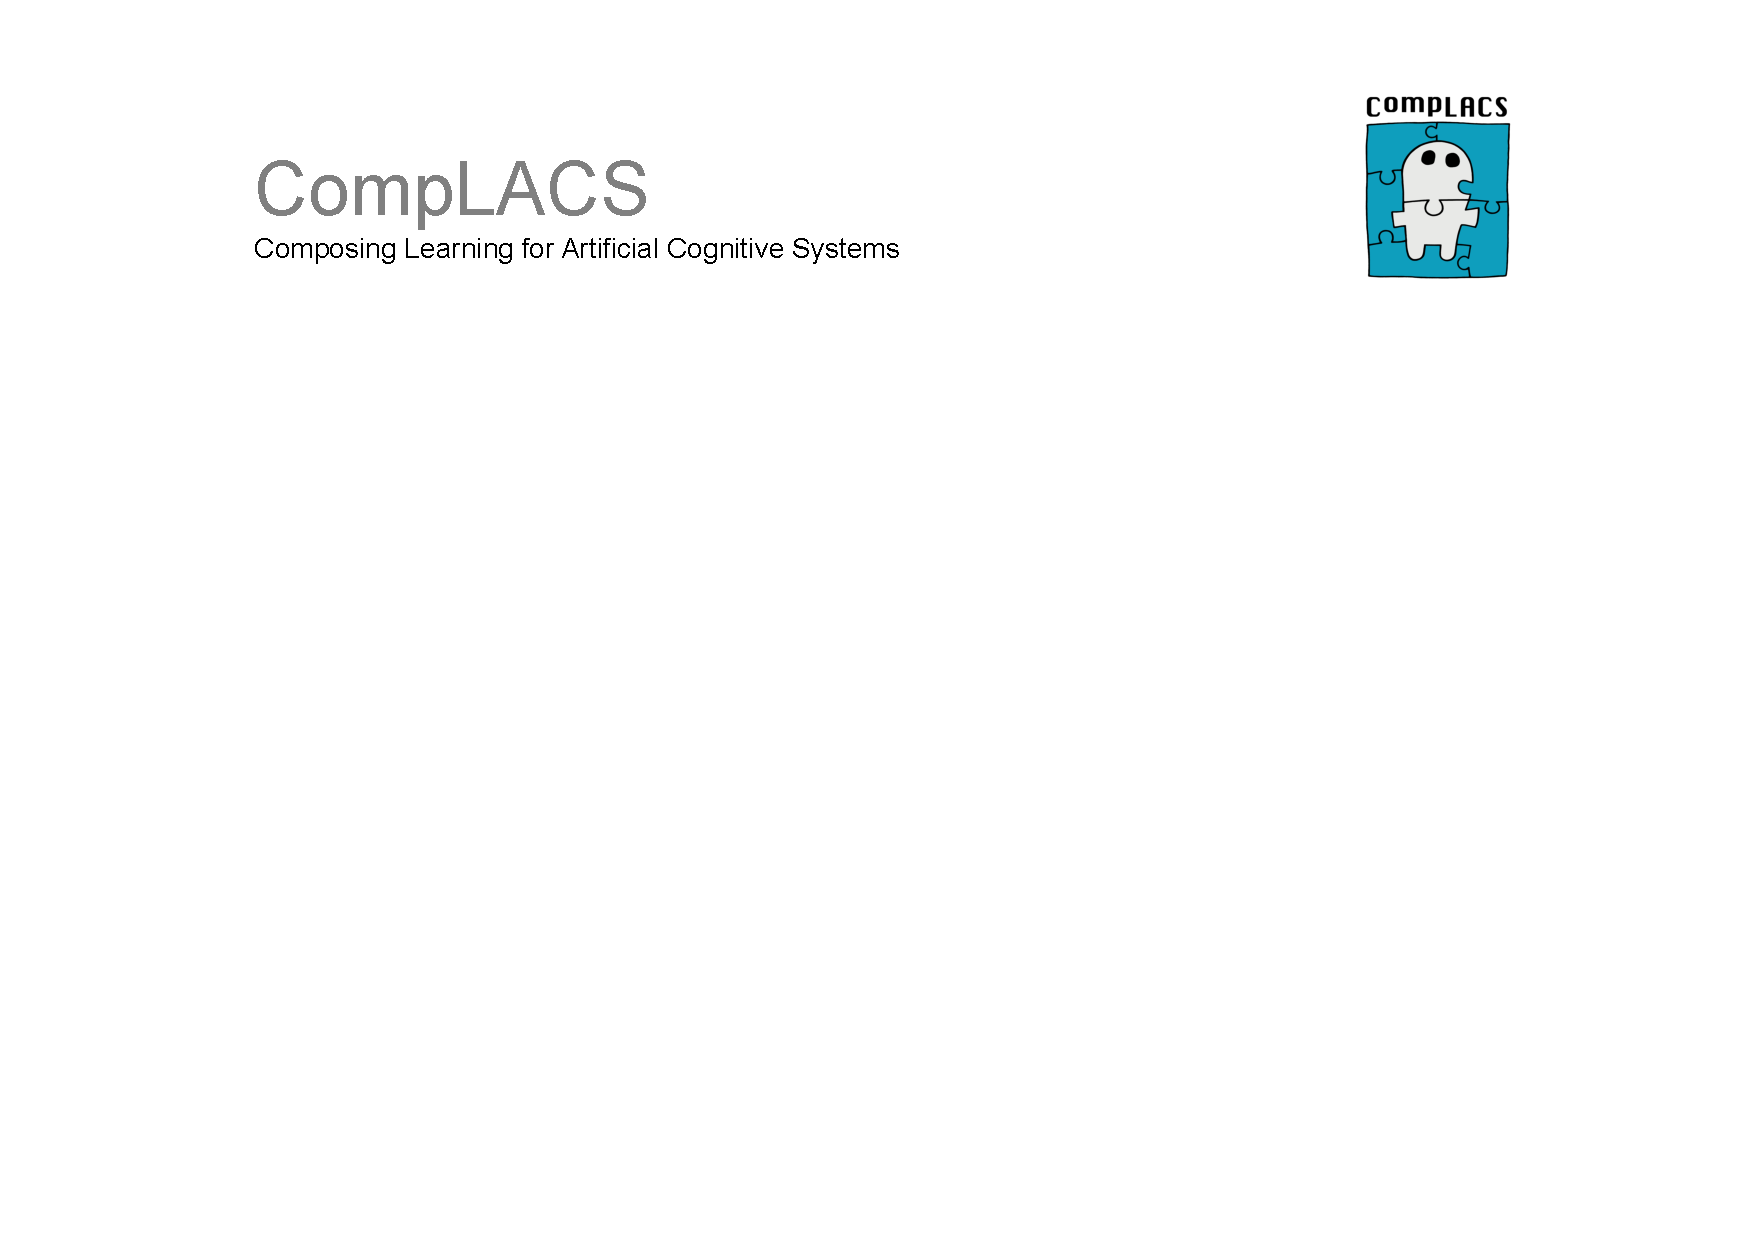
\includegraphics[trim = 35mm 160mm 35mm 15mm, clip, scale=0.48]{complacstemplate.pdf}
\end{center}
\end{figure}
\vspace{-12mm}
\titlepage
  
\end{frame}

\lyxframeend{}\section{Introduction}


\lyxframeend{}\lyxframe{Co-authors}

Joint work with:
\begin{itemize}
\item John Shawe-Taylor 
\item Ronnie Stafford
\item Csaba Szepesv\'{a}ri
\end{itemize}

\lyxframeend{}

\lyxframeend{}\lyxframe{Overview}

System for {\bf model-based reinforcement learning}:
\begin{itemize} 
\item Model MDP transition dynamics using ``conditional mean embeddings'': induces \underline{\bf finite MDP}
\item Optimize policy: policy/value iteration solves finite MDP exactly
\end{itemize}\pause{}
\underline{\bf Related work}: KBRL \cite{KBRL}, ``Kernel CMEs'' \cite{ICMLa}, ``Pseudo-MDPs'' \cite{Yao2012} use finite MDP induced by model. We address some drawbacks:
\begin{itemize}
\item \underline{\bf Compress} the finite MDP to \underline{\bf scale-up planning}\\ 
\item Scale-up model learning: \underline{\bf fast}, \underline{\bf online} using sparse-greedy kernel matching pursuit
\item Model represented in rich RKHS function class
\item Bound value of learned policy in terms of model error
\end{itemize}



\begin{columns}
\column{0.16\linewidth}
%\begin{figure}[hbt]\begin{center}
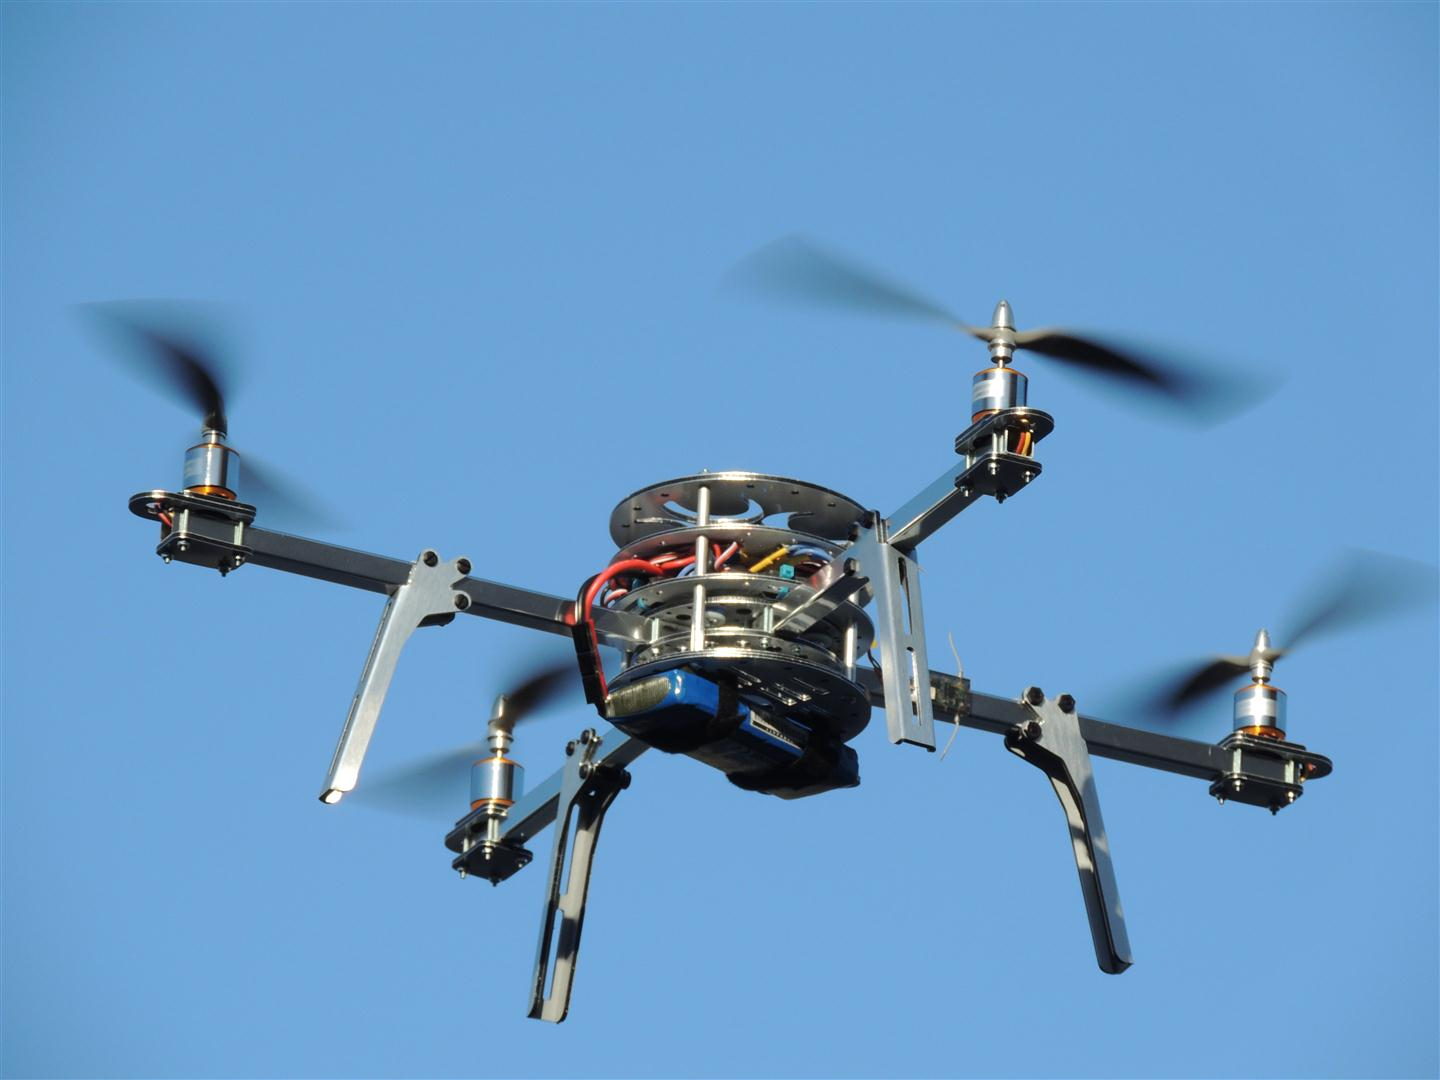
\includegraphics[width=1\textwidth]{quadcoppic}
%\caption{ping pong robot}
%\label{pingpongbot}\end{center}
%\end{figure}
 \column{0.84\linewidth}

Experiments on quadrotor simulator

\end{columns}

\lyxframeend{}






\iffalse
\lyxframeend{}\lyxframe{Related Work}

KBRL \cite{KBRL}, ``Kernel CMEs'' \cite{ICMLa} also use finite MDP induced by model

Advantages:
\begin{itemize}
\item stable (planning via dynamic programming converges)
\item sample efficient
\item performance guarantees/consistency
\end{itemize}\pause{}

We address some drawbacks:
\begin{itemize}
\item Scale-up planning: \underline{\bf compress} the finite MDP for \underline{\bf fast planning}\\ 
\item Scale-up model learning: \underline{\bf fast}, \underline{\bf online} using sparse-greedy kernel matching pursuit
\item Model represented in rich RKHS function class
\end{itemize}

\lyxframeend{}
\fi



\lyxframeend{}\lyxframe{Reinforcement Learning Background}

Reinforcement learning: agent sequentially interacts with unknown environment, receiving rewards\\ 
Formalized as MDP $\cM = \{\cS,\cA,r,P \}$\pause{}
\begin{itemize}
\item $\cS$ state space
\item  $\cA$ action set
\item  $r:\cS\times\cA\to\R$ reward function (known)
\item $P(s'|s,a)$ transition dynamics (Markovian, unknown)
\end{itemize}\pause{}
\emph{Agent} controls trajectory $s_1,a_1,s_2,...$, where $S_{i+1}\sim P(\cdot|s_i,a_i)$, using \emph{policy } $\pi$ where $A_t \sim \pi(\cdot|s_t)$, receives $r(s_t,a_t)$ \\ \pause{}
Goal: find \emph{policy} $\pi^*$ maximizing cumulative reward:
$$J^{\pi}:= \Expect\left[\sum_{t=1}^\infty \gamma^{t-1} r(S_t,A_t) ; \pi \right]$$
\lyxframeend{}





\lyxframeend{}\lyxframe{Reinforcement Learning Background (2)}
\underline{\bf Value function methods} $V^{\pi}(s):= \Expect\left[\sum_{t=1}^\infty \gamma^{t-1} r(S_t,A_t) \bigg| S_1 = s ; \pi \right]$ \pause{}

\emph{policy/value iteration} learns $V^*(s) = \sup_{\pi\in\Pi} V^\pi(s)$
\begin{overprint}
\onslide<2>
$$ V^*(s) =  \max_{a\in\cA} \{r(s,a) + \gamma \Expect_{S' \sim P(\cdot|s,a)}[V^*(S')] \}$$
\onslide<3,4,5>
$$ V_{\textcolor{red}{k+1}}(s) \textcolor{red}{\leftarrow}  \max_{a\in\cA} \{ r(s,a) + \gamma \Expect_{S' \sim P(\cdot|s,a)}[V_{\textcolor{red}{k}}(S')] \} $$
\end{overprint}\pause{}\pause{}
\iffalse
$$ \pi_K(s) := \argmax_{a\in\cA} \{ r(s,a) + \gamma \Expect_{S' \sim P(\cdot|s,a)}[V_K(S')] \} $$\pause{}
Large state spaces need function approximation: e.g.
$$V(s)\approx \lang \bw , \phi(s)\rang _{\cF} $$
usually solve Bellman equations approximately 
\fi



Dynamics unknown $\Rightarrow$ \underline{\bf Model-based RL}\\
\iffalse
\begin{itemize}
\item Collect data from environment $\cD = \{ (s_i, a_i, s'_i) \}_{i=1}^n $
\item Estimate transition dynamics $P(S'|s,a)$ 
\item Plan using the model, in simulation 
\item Repeat
\end{itemize}\pause{}
\fi
\quad-- {\bf Sample efficient}, transfer model to new tasks... 


\lyxframeend{}



\iffalse
\lyxframeend{}\lyxframe{Value iteration cont.}

\vspace{-1cm}
\begin{overprint}
\onslide<3>
$$  V_{k+1}(s) {\leftarrow} \max_{a\in\cA} \{ r(s,a) + \gamma \Expect_{S' \sim P(\cdot|s,a)}[V_{k}(S')|s,a] \} $$
\onslide<4>
$$ \textcolor{red} {\lang \bw_{k+1} , \phi(s) \rang} \leftarrow \max_{a\in\cA} \{ r(s,a) + \gamma \Expect_{S' \sim P(\cdot|s,a)}[\textcolor{red}{\lang \bw_k ,\phi(S') \rang}|s,a] \}  $$
\onslide<5,6,7>
$$  \lang \bw_{k+1} , \phi(s) \rang \textcolor{red}{!\leftarrow} \max_{a\in\cA} \{ r(s,a) + \gamma \Expect_{S' \sim P(\cdot|s,a)}[\lang \bw_k ,\phi(S') \rang|s,a] \}$$
\end{overprint}\pause{}\pause{}\pause{}
Approximate setting: Bellman map and projection not contraction
\begin{align}
\lang \bw_{k+1} , \phi(s) \rang \textcolor{red}{\approx} \sup_{a\in\cA} \{ r(s,a) + \gamma \Expect_{S' \sim P(\cdot|s,a)}[\lang \bw_k ,\phi(S') \rang|s,a] \}  \nn 
\end{align}\pause{}

\textcolor{red}{We will present an approximate value iteration algorithm which converges}

\lyxframeend{}
\fi

\iffalse
\lyxframeend{}\lyxframe{Model-based RL}

Policy/value iteration requires knowledge of dynamics $P(S'|s,a)$, but \textcolor{red}{unknown} \\ \pause{}

Model-based RL:
\begin{itemize}
\item Collect data from environment 
\begin{align}
\cD = \{ (s_i, a_i, s'_i) \}_{i=1}^n  \quad\quad s'_i \sim P(\cdot|s_i,a_i) \nn 
\end{align}
\item Estimate transition dynamics $P(S'|s,a)$ 
\item Plan using the model, in simulation 
\item Repeat
\end{itemize}\pause{}

Advantages:
\begin{itemize}
\item {\bf Sample efficient} -- minimize interactions with environment
\item Model may transfer to different tasks
\end{itemize}

\lyxframeend{}
\fi










\iffalse
\lyxframeend{}\lyxframe{Model-based RL (3): Types of model}



We need: $\Expect_{S' \sim P(\cdot|s,a)}[V^\pi(S')|s,a] \approx  \lang \bw_\pi,  \Expect_{S' \sim P(\cdot|s,a)}[\phi(S')] \rang$\pause{}
Conditional Density estimation
\begin{itemize}
\item Estimate conditional density $\hat P(S'|s,a) \approx P(S'|s,a)$
\item Integrate: $\Expect_{S' \sim P(\cdot|s,a)}[V^\pi(S')] \approx \int \hat P(s'|s,a) V(s') ds'$
\end{itemize} \pause{}

Linear models \textcolor{red}{per policy}
\begin{itemize}
\item Learn function $\mu_\pi:s\to \Expect[\phi(S')|s,\pi(s)] $
\item $\mu_\pi(s) = \bB_\pi \phi(s) \approx \Expect[\phi(S')|s,\pi(s)]$ e.g. least squares
\item Implicitly in approximate policy iteration with LSTD
\item Not off-policy! Wasteful
\end{itemize} \pause{}

Linear models \textcolor{red}{per action}
\begin{itemize}
\item Learn functions $\mu_a:s\to \Expect[\phi(S')|s,a]$
\item Can we generalize between actions?
\end{itemize}

\lyxframeend{}
\fi




\lyxframeend{}\section{Modelling Dynamics with Compressed CMEs}


\lyxframeend{}\lyxframe{Model Dynamics with Kernel CMEs}

What do we need from a model? Consider generalized linear value representation $V_{k}(s) \approx \lang w_k ,  \phi(s) \rang_{\cF}$
\begin{overprint}
\onslide<1>
$$ V_{k+1}(s) {\leftarrow}  \max_{a\in\cA} \{ r(s,a) + \gamma \Expect_{S' \sim P(\cdot|s,a)}[V_{k}(S')] \} $$
\onslide<2,3,4>
$$ V_{k+1}(s) {\leftarrow}  \max_{a\in\cA} \{ r(s,a) + \gamma \lang w_k ,  \textcolor{red}{\Expect_{S' \sim P(\cdot|s,a)}[\phi(S')]}\rang_{\cF} \}  $$
\end{overprint}\pause{}\pause{}
We need to learn \underline{\bf ``conditional mean embedding''}
$$\mu(s,a):= \textcolor{red}{\Expect_{S' \sim P(\cdot|s,a)}[\phi(S')]}$$
No generative model, no density, no sampling\\\pause{}
\iffalse
We suppose $V^*\in\cH_L$ for some RKHS $\cH_L$ with kernel $L$\\ \pause{}
Implicitly $\phi(s) = L(s,\cdot)$ but $\cH_L$ very rich class\\ \pause{}
\begin{enumerate}
\item We learn the function $\mu: \cS\times\cA\to\cH_L$:
\begin{align}
\mu: (s,a) \to \Expect_{S' \sim P(\cdot|s,a)}[L(S',\cdot)],\nn
\end{align}\pause{} 
Note then by \textcolor{red}{reproducing property of $L$}
\begin{align}
\Expect_{S' \sim P(\cdot|s,a)}[V(S')] &= \lang V(\cdot) , \Expect_{S' \sim P(\cdot|s,a)}[L(S',\cdot)] \rang_L \nn \\
 &= \lang V(\cdot) , \mu(s,a) \rang_L \nn 
\end{align}\pause{}

\item Incorporate model into policy/value iteration\\
\end{enumerate} \pause{}
$\mu$ called \textcolor{red}{\emph{conditional mean embedding}} (CME) of $P(S'|S,A)$ in $\cH_L$
\fi
Incorporate approximate model $\hat \mu \approx \mu$ into policy/value iteration

\lyxframeend{}






\lyxframeend{}\lyxframe{Learning CMEs}
Given system data, $\cD = \{ (s_i, a_i), \phi(s'_i) \}_{i=1}^n$, find
$$\hat \mu = \argmin_{\mu:\cS\times\cA\to\cF} \sum_{i=1}^n ||\phi(s'_i) - \mu(s_i,a_i)||_\cF^2$$\pause{}
e.g. kernel smoothing (KBRL), kernel least-squares\\ \pause{}

\underline{\bf Induced Finite MDP}:\\
Models have form $\hat \mu(s,a) :=  \sum_{j=1}^n \alpha_j(s,a)\phi(s'_j)$ so
\begin{align}
\Expect[V(S')|s,a] &\approx  \sum_{i=1}^n \alpha_i(s,a) V(s'_i)\nn
\end{align}\pause{}
i.e. we only need to \underline{maintain $V$ on samples}\\ \pause{}

If $||\alpha(s,a)||_1\le 1$, $\alpha_i(s,a)$, \underline{plan exactly on finite (pseudo-)MDP}...

\lyxframeend{}




\lyxframeend{}\lyxframe{Algorithm: Online Policy Optimization with CME model}

Repeat:

{1:} Update data $\cD = \{ (s_i, a_i, s'_i) \}_{i=1}^n$\\
{2:} Update dynamics model $\hat\mu(s,a) = \sum_{j=1}^n \alpha_j(s,a)\phi(s'_j)$\\
{3:} Value iteration with approximate model: for $s\in\{s'_1,...,s'_n\}$
%\vspace{-3mm}
\begin{align}
V_{k+1}(s) &\leftarrow \max_{a\in\cA} \{ r(s,a) + \gamma \Expect_{S' \sim P(\cdot|s,a)}[ V_{k}(S')] \} \nn\\
&\approx \max_{a\in\cA} \{ r(s,a) + \gamma \sum_{j=1}^n \alpha_j(s,a) V_{k}(s'_j) \} \nn
\end{align}
%\vspace{-3mm}
{4:} Act greedily $\pi_K(s) \hspace{-1mm}=\hspace{-1mm} \argmax_{a\in\cA} \{ r(s,a)\hspace{-1mm} +\hspace{-1mm} \gamma \sum_{j=1}^n \alpha_j(s,a) V_{K}(s'_j) \}$\\ \pause{}
\underline{\bf Advantages}: value iteration converges; avoid approx. dynamic programming; good performance bounds\\
\underline{\bf Problems}: planning scales poorly $O(|\cA|kn^2)$; model learning can be slow




\lyxframeend{}



\lyxframeend{}\lyxframe{Fast Planning with a Compressed Model}

Compress the induced MDP without losing performance:\\

Maintain a ``$\delta$-lossy compression'' $\cC = \{ c_1,...,c_m\}$ of $\{s'_1,...,s'_n\}$ s.t.

$$\max_{1\le j \le n} \min_{b:||b||_1\le 1} ||\sum_{i=1}^m b_i \phi(c_i) - \phi(s'_j)||_\cF\le \delta$$\pause{}

Represent $\hat\mu$ on $\cC$: $\hat\mu(s,a) = \sum_{j=1}^m \alpha_i(s,a)\phi(c_j)$: \underline{\bf planning $O(|\cA|km^2)$} \\ \pause{}
Algorithm: \texttt{augmentCompressionSet}$(\cC,\delta,s)$\vspace{-4mm}
%\begin{algorithm}
%   \caption{\texttt{augmentCompressionSet}$(\cC,\delta,s)$}
\begin{algorithmic}
   \STATE {\bf Input:}  Initial compression set $\cC = {c_1,...,c_m}$, candidate $s\in\cS$, tolerance $\delta$
	 \IF {$\min_{{\bm b}\in\R^m , ||{\bm b}||_1\le 1}\hspace{-0.6mm} ||\sum_{i=1}^m b_i \phi(c_i) \hspace{-0.6mm}-\hspace{-0.6mm} \phi(s)||_{\cF} \hspace{-0.6mm}>\hspace{-0.6mm} \delta$}
	 \STATE {\bf Augment:} $\cC \leftarrow \cC \cup s$
	\ENDIF
\end{algorithmic}
%\end{algorithm}
minimization is a Lasso

\lyxframeend{}


\iffalse
\lyxframeend{}\lyxframe{Performance guarantees for Compressed Model}


Guarantees on the performance of the learnt policy \cite{ICMLa}:\vspace{-0.5cm}\pause{}
\begin{overprint}
\onslide<2>
\begin{theorem}
\begin{align}
||V^{\pi_k} - V^*||_{\infty} &\le \frac{2\gamma}{(1-\gamma)^2} \big(  \gamma^k||V^{\pi_1} - V^{\pi_0}||_\infty + 2||V^* - \tilde V^*||_{\infty} \nn\\
& +\sup_{s,a}||\Expect_{S'\sim P(\cdot|s,a)}[\phi(S')] - \hat \mu(s,a)||_\cF ||\tilde V^*||_\cF \big)\nn
\end{align}
\end{theorem}
\begin{itemize}
\item $V^{\pi_k}$ value of learnt policy after $k$ steps
\item $V^*$ value of optimal policy
\item $\tilde V^*$ arbitrary element in $\cF$
\item error from value iteration $+$ approximation error $+$ embeddings estimation error
\end{itemize}
\onslide<3>
\begin{theorem}
\begin{align}
||V^{\pi_k} - V^*||_{\infty} &\le \frac{2\gamma}{(1-\gamma)^2} \big( {\cred \gamma^k||V^{\pi_1} - V^{\pi_0}||_\infty} + 2||V^* - \tilde V^*||_{\infty} \nn\\
& +\sup_{s,a}||\Expect_{S'\sim P(\cdot|s,a)}[\phi(S')] - \hat \mu(s,a)||_\cF ||\tilde V^*||_\cF \big)\nn
\end{align}
\end{theorem}
\begin{itemize}
\item $V^{\pi_k}$ value of learnt policy after $k$ steps
\item $V^*$ value of optimal policy
\item $\tilde V^*$ arbitrary element in $\cF$
\item {\cred error from value iteration} $+$ approximation error $+$ embeddings estimation error
\end{itemize}
\onslide<4>
\begin{theorem}
\begin{align}
||V^{\pi_k} - V^*||_{\infty} &\le \frac{2\gamma}{(1-\gamma)^2} \big(  \gamma^k||V^{\pi_1} - V^{\pi_0}||_\infty + {\cred 2||V^* - \tilde V^*||_{\infty}} \nn\\
& +\sup_{s,a}||\Expect_{S'\sim P(\cdot|s,a)}[\phi(S')] - \hat \mu(s,a)||_\cF ||\tilde V^*||_\cF \big)\nn
\end{align}
\end{theorem}
\begin{itemize}
\item $V^{\pi_k}$ value of learnt policy after $k$ steps
\item $V^*$ value of optimal policy
\item $\tilde V^*$ arbitrary element in $\cF$
\item error from value iteration $+$ {\cred approximation error} $+$ embeddings estimation error
\end{itemize}
\onslide<5>
\begin{theorem}
\begin{align}
||V^{\pi_k} - V^*||_{\infty} &\le \frac{2\gamma}{(1-\gamma)^2} \big(  \gamma^k||V^{\pi_1} - V^{\pi_0}||_\infty +  2||V^* - \tilde V^*||_{\infty} \nn\\
& +{\cred\sup_{s,a}||\Expect_{S'\sim P(\cdot|s,a)}[\phi(S')] - \hat \mu(s,a)||_\cF ||\tilde V^*||_\cF} \big)\nn
\end{align}
\end{theorem}
\begin{itemize}
\item $V^{\pi_k}$ value of learnt policy after $k$ steps
\item $V^*$ value of optimal policy
\item $\tilde V^*$ arbitrary element in $\cF$
\item error from value iteration $+$ approximation error $+$  {\cred embeddings estimation error}
\end{itemize}
\end{overprint}\pause{}\pause{}\pause{}

\lyxframeend{}

\fi




\lyxframeend{}\lyxframe{Performance guarantees for Compressed Model}
\vspace{-4mm}
\begin{overprint}
\onslide<1,5>
\begin{theorem}
Bound for value iteration with CME $\hat \mu$: for any $\tilde V^* \in \cF$\vspace{-3mm}
\begin{align}
||V^{\pi_k} - V^*||_{\infty} &\le \frac{2\gamma}{(1-\gamma)^2} \big(  \gamma^k||V^{\pi_1} - V^{\pi_0}||_\infty + 2||V^* - \tilde V^*||_{\infty} \nn\\
& +\sup_{s,a}||\Expect_{S'\sim P(\cdot|s,a)}[\phi(S')] - \hat \mu(s,a)||_\cF ||\tilde V^*||_\cF \big)\nn\\
&=:B_k(\hat \mu) \nn
\end{align}
\end{theorem}
\onslide<2>
\begin{theorem}
Bound for value iteration with CME $\hat \mu$: for any $\tilde V^* \in \cF$\vspace{-3mm}
\begin{align}
||V^{\pi_k} - V^*||_{\infty} &\le \frac{2\gamma}{(1-\gamma)^2} \big( {\cred \gamma^k||V^{\pi_1} - V^{\pi_0}||_\infty} + 2||V^* - \tilde V^*||_{\infty} \nn\\
& +\sup_{s,a}||\Expect_{S'\sim P(\cdot|s,a)}[\phi(S')] - \hat \mu(s,a)||_\cF ||\tilde V^*||_\cF \big)\nn\\
&=:B_k(\hat \mu) \nn
\end{align}
\end{theorem}
\onslide<3>
\begin{theorem}
Bound for value iteration with CME $\hat \mu$: for any $\tilde V^* \in \cF$\vspace{-3mm}
\begin{align}
||V^{\pi_k} - V^*||_{\infty} &\le \frac{2\gamma}{(1-\gamma)^2} \big(  \gamma^k||V^{\pi_1} - V^{\pi_0}||_\infty + {\cred 2||V^* - \tilde V^*||_{\infty}} \nn\\
& +\sup_{s,a}||\Expect_{S'\sim P(\cdot|s,a)}[\phi(S')] - \hat \mu(s,a)||_\cF ||\tilde V^*||_\cF \big)\nn\\
&=:B_k(\hat \mu) \nn
\end{align}
\end{theorem}
\onslide<4>
\begin{theorem}
Bound for value iteration with CME $\hat \mu$: for any $\tilde V^* \in \cF$\vspace{-3mm}
\begin{align}
||V^{\pi_k} - V^*||_{\infty} &\le \frac{2\gamma}{(1-\gamma)^2} \big(  \gamma^k||V^{\pi_1} - V^{\pi_0}||_\infty +  2||V^* - \tilde V^*||_{\infty} \nn\\
& +{\cred\sup_{s,a}||\Expect_{S'\sim P(\cdot|s,a)}[\phi(S')] - \hat \mu(s,a)||_\cF ||\tilde V^*||_\cF} \big)\nn\\
&=:B_k(\hat \mu) \nn
\end{align}
\end{theorem}
\end{overprint}\pause{}\pause{}\pause{}\pause{}


\begin{theorem}
If $\hat \mu$ defined on $\{s'_1,...,s'_n\}$ and $\cC$ a $\delta$-lossy compression, then there exists $\bar \mu$ represented on $\cC$ such that after $k$ value iterations using $\bar \mu$
\begin{align}
||V^{\pi_k} - V^*||_{\infty} &\le B_k(\hat \mu)  +\frac{2\gamma\delta}{(1-\gamma)^2}||\tilde V^*||_\cF\nn
\end{align}
\end{theorem}


\lyxframeend{}




\iffalse

\lyxframeend{}\lyxframe{Performance guarantees for Compressed Model}

\begin{theorem}
Standard bound for any $\hat \mu$ \vspace{-3mm}
\begin{align}
||V^{\pi_k} - V^*||_{\infty} &\le \frac{2\gamma}{(1-\gamma)^2} \big(  \gamma^k||V^{\pi_1} - V^{\pi_0}||_\infty + 2||V^* - \tilde V^*||_{\infty} \nn\\
& +\sup_{s,a}||\Expect_{S'\sim P(\cdot|s,a)}[\phi(S')] - \hat \mu(s,a)||_\cF ||\tilde V^*||_\cF \big)\nn\\
&=:B_k(\hat \mu) \nn
\end{align}
\end{theorem}

\begin{theorem}
If $\hat \mu$ defined on $\{s'_1,...,s'_n\}$ and $\cC$ a $\delta$-lossy compression, then there exists $\bar \mu$ represented on $\cC$ such that after $k$ value iterations using $\bar \mu$
\begin{align}
||V^{\pi_k} - V^*||_{\infty} &\le B_k(\hat \mu)  +\frac{2\gamma\delta}{1-\gamma^2}||\tilde V^*||_\cF\nn
\end{align}
\end{theorem}

\lyxframeend{}

\fi


\lyxframeend{}\lyxframe{Fast Model Learning with Matching Pursuit}

Optimize the model: Kernel smoothing, Kernel least-squares?\\\pause{}

We use the (vector-valued) kernel regressor: put kernel $K$ on input space $\cS\times \cA$, 
\begin{align}
\hat \mu(s,a) :=  \sum_{i=1}^n\sum_{j=1}^m K((s,a),(s_i,a_i))W_{ij}\phi(c_j), \nn
\end{align}
Learn $\bW$ by \underline{\bf sparse-greedy} kernel matching pursuit: 
\begin{itemize}
\item \underline{\bf fast}, \underline{\bf online} and $\bW$ row sparse.
\item models dynamics in rich kernel-defined RKHS $\cH_K$\
\end{itemize}

Project: $\alpha(s,a) = \argmin{\beta:||\beta||_1\le 1} \{ ||\sum_{j=1}^m \beta_j(s,a)\phi(s_j') - \sum_{i=1}^n \sum_{j=1}^m K((s,a),(s_i,a_i))W_{ij}\phi(c'_j) ||^2_\cF \}$ (Lasso)

\lyxframeend{}





\iffalse
\lyxframeend{}\lyxframe{Convergence Guarantee}

Approximate value iteration converges (rare!)

\begin{itemize}
\item $\hat \mu(s,a)  = \sum_{i=1}^m \alpha_i(s,a) L(s'_i,\cdot)$
\item If we normalize $\bar \alpha_i(s,a)$ s.t. $\sum_i |\bar\alpha_i(s,a)|\le 1$ then 
$$\hat T^*: V \mapsto \sup_{a\in\cA} \{ r(s,a) +  \gamma \lang V_{k}(\cdot), \hat \mu(s,a)\rang_L \}$$
is a contraction
\item \cite{Yao2012} Present a way to add this constraint to the optimization (but unneccesary in the limit anyway)
\end{itemize}

\lyxframeend{}
\fi


\iffalse
\lyxframeend{}\lyxframe{Work on samples}


Useful property of the kernel approach:
\begin{align}
\Expect[V_k(S'|s,a)] &\approx\lang V_{k}(\cdot), \hat \mu(s,a)\rang_L \nn\\
&= \sum_{i=1}^m \alpha_i(s,a) V_k(s'_i)\nn
\end{align}\pause{}
\textcolor{red}{i.e. we only need to know $V$ on the samples!}\\ \pause{}
$$ V_{k+1}(s_j') \leftarrow \sup_{a\in\cA} \{ r(s_j',a) + \gamma \sum_{i=1^m} \alpha_i(s'_j,a)V_{k}(s_i') \} $$\pause{}
$O(|\cD|^2 k |\cA|)$\\ \pause{}
Consequence of reproducing property and representer theorem 

\lyxframeend{}
\fi













\lyxframeend{}\section{Experiments and Conclusion}


\lyxframeend{}\lyxframe{Experiments}

Mountain Car and Cart-Pole benchmark MDPs: rewards

\begin{figure}[htp]
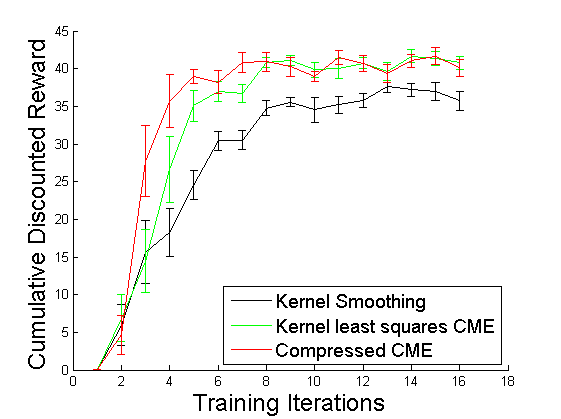
\includegraphics[clip, scale=0.20]{MCrewardsb.png}
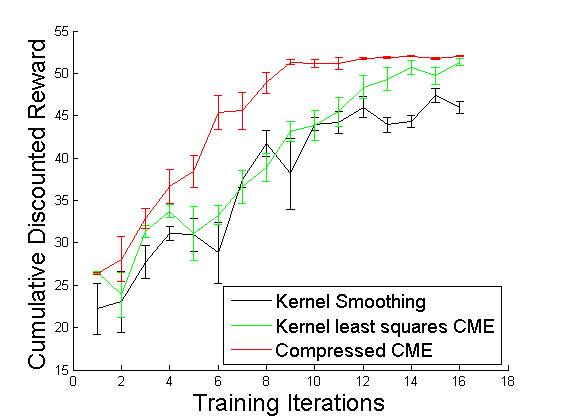
\includegraphics[clip, scale=0.20]{CPrewardsb.png}

  \label{rewardPlot}
\end{figure}

\underline{\bf faster planning} using compact data-defined representation

\begin{figure}[htp]
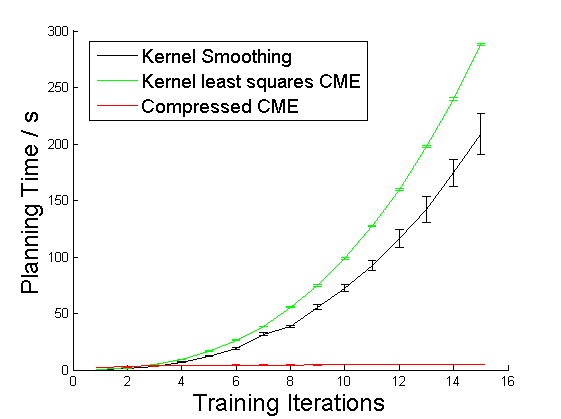
\includegraphics[clip, scale=0.20]{MCplanningb.png}
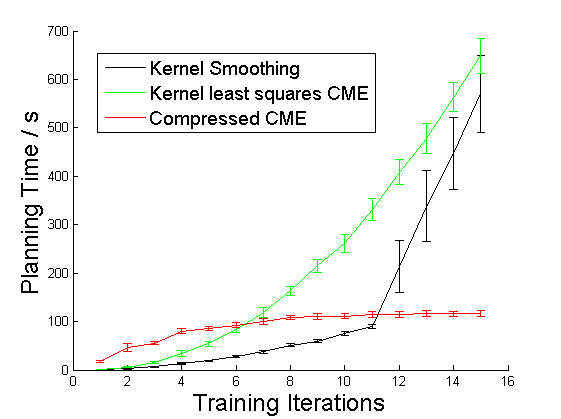
\includegraphics[clip, scale=0.20]{CPplanningb.png}

  \label{planningPlot}
\end{figure}\pause{}

Simulated quadrotor experiments, $dim(\cS)=13$.

\lyxframeend{}




\lyxframeend{}\lyxframe{Conclusions}
A system for general reinforcement learning:
\begin{itemize}
\item Learn system transition dynamics using CME
\item Compress the model for fast planning
\item Rich, data-dependent, RKHS model class
\item Optimize policy with value/policy iteration on induced finite MDP
\item Performance guarantee
\end{itemize}

Future work
\begin{itemize}
\item Represent $\mu(s,a)$ using neural nets
\item Connection to subgoals
\end{itemize}



\lyxframeend{}

\lyxframeend{}\lyxframe{References}
\begin{footnotesize}
 \begin{thebibliography}{10}  
 %\beamertemplatearticlebibitems
  \bibitem{ICMLa}
     S.~Grunewalder, G.~Lever, L.~Baldessarre, M.~Pontil, A.~Gretton
    \newblock {\em Modelling transition dynamics in MDPs with RKHS embeddings}.
    \newblock ICML 2012.  
		
	%\beamertemplatearticlebibitems
  \bibitem{KBRL}
     D.~Ormoneit, S.~Sen
    \newblock {\em Kernel-based reinforcement learning}.
    \newblock Machine Learning 2002.  
    
  \bibitem{Yao2012}
     H.~Yao, Cs.~Szepesv\'{a}ri, B.A.~Pires and X.~Zhang
    \newblock {\em Pseudo-MDPs and Factored Linear Action Models}.
    \newblock IEEE ADPRL, 2014.


  \end{thebibliography}
	\end{footnotesize}

\lyxframeend{}



\end{document}